\chapter{Machine Learning Pipeline}

% ==========================================
% SECTION 1: ML PIPELINE
% ==========================================
\section{Quy trình Machine Learning (ML Pipeline)}

\begin{figure}[H]
    \centering
    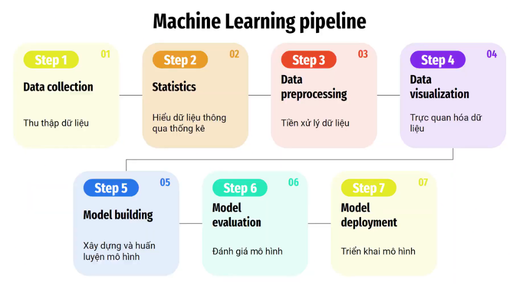
\includegraphics[width=0.8\linewidth]{11.png}
    %\fbox{\parbox[c][4cm][c]{0.8\linewidth}{\centering \textit{[Chèn ảnh: Tổng quan ML Pipeline tại đây]}}}
    \caption{Quy trình tổng quan của một ML Pipeline}
    \label{fig:ml_pipeline}
\end{figure}

\subsection{Step 1: Data Collection (Thu thập dữ liệu)}
\begin{itemize}
    \item Xác định bài toán và dữ liệu cần có.
    \item Thu thập dữ liệu.
    \item Đánh nhãn (Annotation).
    \item \textbf{OUTPUT:} Dữ liệu thô (Raw data).
\end{itemize}

\subsection{Step 2: Statistics (Thống kê mô tả)}
\begin{itemize}
    \item Thống kê: Tính toán các thông số cơ bản:
    \begin{itemize}
        \item \textbf{Mean:} Trung bình.
        \item \textbf{Median:} Trung vị.
        \item \textbf{Std:} Độ lệch chuẩn.
        \item \textbf{Variance:} Phương sai.
        \item \textbf{Min/Max:} Giá trị nhỏ nhất / lớn nhất.
        \item \textbf{Q1, Q2, Q3:} Tứ phân vị.
        \item \textbf{Mode:} Điểm dữ liệu có tần số xuất hiện lớn nhất.
    \end{itemize}
    \item \textbf{OUTPUT:} Cung cấp cái nhìn tổng quan về bộ dữ liệu.
\end{itemize}

\subsection{Step 3: Data Preprocessing (Tiền xử lý dữ liệu)}
\begin{itemize}
    \item Đưa dữ liệu về dạng máy tính có thể hiểu được (dạng số).
    \item Làm sạch dữ liệu.
    \item Chuẩn hóa: Đưa mọi tham số về cùng một thang đo.
    \item Phân chia dữ liệu: Training set, Validation set, Test set.
    \item Tạo đặc trưng mới dựa trên dữ liệu sau xử lý.
    \item Các bước trong quá trình này được xây dựng và mô hình hóa thành một pipeline/mô hình riêng, phục vụ cho các pha khác để đảm bảo tính thống nhất.
    \item \textbf{OUTPUT:} Dữ liệu đã được làm sạch, chuẩn hóa và phân chia thành từng cụm phục vụ cho từng bước.
\end{itemize}

\subsection{Step 4: Data Visualization (Trực quan hóa dữ liệu)}
\begin{itemize}
    \item Dựa trên dữ liệu cung cấp, cần trực quan hóa dữ liệu để có thể dễ dàng quan sát.
    \item Sử dụng các thư viện của python.
    \item \textbf{OUTPUT:} Biểu đồ.
\end{itemize}

\subsection{Step 5: Model Building (Xây dựng mô hình)}
\begin{itemize}
    \item Chọn thuật toán phù hợp.
    \item Tiến hành training dựa trên Training set.
    \item \textbf{Tinh chỉnh} các tham số dựa trên kết quả đầu ra.
    \item Sử dụng thêm các mô hình khác để so sánh.
    \item \textbf{OUTPUT:} Trả về mô hình đã huấn luyện, có thể dùng để dự đoán.
\end{itemize}

\subsection{Step 6: Model Evaluation (Đánh giá mô hình)}
\begin{itemize}
    \item Từ kết quả thu được trên Test set, tính toán các thông số như: Accuracy, Precision, Recall, F1 score, ROC, AUC.
    \item Kiểm tra hiện tượng Overfitting (Train tốt, Test kém).
    \item Tiến hành đánh giá kết quả của mô hình sau bài test.
    \item \textbf{OUTPUT:} Dựa vào kết quả để kết luận mô hình có đạt không. Nếu không đạt, cần xác định quay lại bước nào để tinh chỉnh.
\end{itemize}

\subsection{Step 7: Model Deployment (Triển khai mô hình)}
\begin{itemize}
    \item Tích hợp, triển khai mô hình vào các thiết bị, cloud,... để sử dụng tùy vào mục đích.
\end{itemize}

\subsection{Lưu ý về vòng lặp của Pipeline}
\begin{figure}[H]
    \centering
    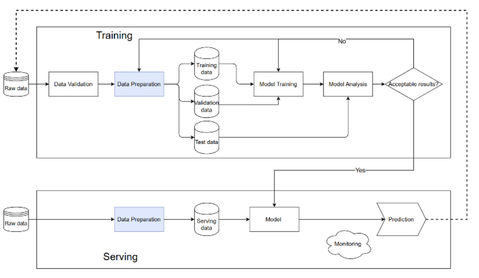
\includegraphics[width=0.8\linewidth]{12.png}
    \caption{Machine learning pipeline}
    \label{fig: hieuchinh}
\end{figure}
\begin{itemize}
    \item Pipeline thường \textbf{không chạy một chiều}, cần phải cải thiện lại nếu Step 6 chưa đạt kết quả như kỳ vọng.
    \item Đường đi phản hồi: $\text{Prediction} \rightarrow \text{Raw data}$.
    \item Nghĩa là dữ liệu thu được từ mô hình được đưa ngược về để làm Training set nhằm đảm bảo mô hình có thể bắt kịp với những thay đổi thực tế.
\end{itemize}

% ==========================================
% SECTION 2: CHI TIẾT TIỀN XỬ LÝ DỮ LIỆU
% ==========================================
\section{Các bước Tiền xử lý dữ liệu (Data Preprocessing)}

\begin{figure}[H]
    \centering
    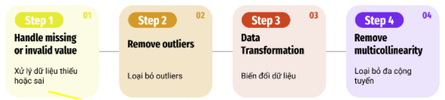
\includegraphics[width=0.8\linewidth]{13.png}
    %\fbox{\parbox[c][4cm][c]{0.8\linewidth}{\centering \textit{[Chèn ảnh: Quy trình Data Preprocessing tại đây]}}}
    \caption{Các bước chính trong tiền xử lý dữ liệu}
    \label{fig:data_preprocessing}
\end{figure}

\begin{itemize}
    \item \textbf{Step 1:} Handle missing or invalid values (Xử lý dữ liệu thiếu hoặc không hợp lệ).
    \item \textbf{Step 2:} Remove outliers (Loại bỏ các điểm ngoại lai).
    \item \textbf{Step 3:} Data transformation (Biến đổi dữ liệu):
    \begin{itemize}
        \item \textbf{Numerical feature} (Thuộc tính dạng số):
        \begin{itemize}
            \item Tiền xử lý: \texttt{MinMaxScaler} (nhạy cảm với outliers), \texttt{StandardScaler}.
            \item \textbf{Continuous:} Dữ liệu liên tục.
            \item \textbf{Discrete:} Dữ liệu rời rạc.
        \end{itemize}
        \item \textbf{Categorical feature} (Thuộc tính dạng phân loại):
        \begin{itemize}
            \item \textbf{Ordinal} (Thứ bậc) $\rightarrow$ \texttt{OrdinalEncoder}.
            \item \textbf{Nominal} (Danh nghĩa) $\rightarrow$ One-hot encoding, Hash encoding, Word Embedding.
        \end{itemize}
    \end{itemize}
    \begin{figure}[H]
    \centering
    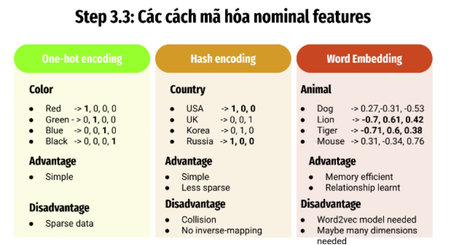
\includegraphics[width=0.8\linewidth]{14.png}
    %\fbox{\parbox[c][4cm][c]{0.8\linewidth}{\centering \textit{[Chèn ảnh: Minh họa Correlation / Multicollinearity tại đây]}}}
    \caption{Các cách mã hóa}
    \label{fig:encoder}
\end{figure}
    \item \textbf{Step 4:} Remove multicollinearity (Loại bỏ hiện tượng đa cộng tuyến).
\end{itemize}

% ==========================================
% SECTION 3: TƯƠNG QUAN & ĐA CỘNG TUYẾN
% ==========================================
\section{Mối quan hệ giữa các biến}

\begin{figure}[H]
    \centering
    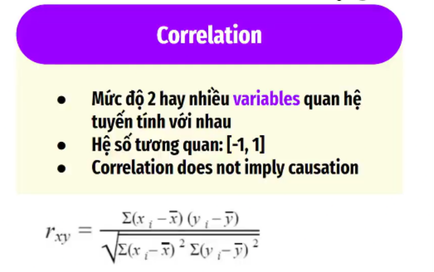
\includegraphics[width=0.8\linewidth]{15.png}
    %\fbox{\parbox[c][4cm][c]{0.8\linewidth}{\centering \textit{[Chèn ảnh: Minh họa Correlation / Multicollinearity tại đây]}}}
    \caption{Minh họa hệ số tương quan $R_{xy}$}
    \label{fig:correlation}
\end{figure}

\subsection{Correlation (Tương quan)}
\begin{itemize}
    \item Đại lượng thống kê biểu thị mức độ mà 2 hay nhiều biến thay đổi cùng nhau một cách tuyến tính.
    \item $R_{xy}$: Hệ số tương quan, có miền giá trị $R_{xy} \in [-1, 1]$:
    \begin{itemize}
        \item $R_{xy} > 0$: Tương quan dương (2 biến cùng tăng hoặc cùng giảm).
        \item $R_{xy} < 0$: Tương quan âm (1 biến tăng, 1 biến giảm).
        \item $R_{xy} = 1$: Tương quan dương hoàn hảo.
        \item $R_{xy} = -1$: Tương quan âm hoàn hảo.
        \item $R_{xy} = 0$: Hai biến không có quan hệ tuyến tính với nhau (nhưng \textbf{không thể} kết luận chúng độc lập).
    \end{itemize}
    \item Hệ số tương quan cho biết mức độ tương quan hay mối quan hệ bậc 1 (tuyến tính) giữa hai biến với nhau.
    \item Tương quan mạnh hay yếu phụ thuộc vào độ lớn của giá trị ($|R_{xy}|$ càng lớn thì các điểm dữ liệu càng nằm gần đường phù hợp nhất).
    \item \textbf{Lưu ý:} Hệ số tương quan \textbf{không thể} suy ra quan hệ nhân quả.
\end{itemize}

\subsection{(Multi)collinearity (Cộng tuyến / Đa cộng tuyến)}
\begin{itemize}
    \item Là mối quan hệ giữa các \textbf{feature} với nhau (phạm vi hẹp hơn correlation).
    \item Trong bài toán:
    \begin{itemize}
        \item \textbf{Feature:} Independent variable (biến độc lập).
        \item \textbf{Target:} Dependent variable (biến phụ thuộc, giống kiểu outcome / kết luận đầu ra).
    \end{itemize}
    \item Đa cộng tuyến là hiện tượng có lúc cần loại bỏ, có lúc không cần.
    \item Phát hiện đa cộng tuyến bằng cách tính hệ số tương quan giữa các feature.
    \item \textbf{Mục tiêu mong muốn:}
    \begin{itemize}
        \item Đối với \textbf{target và feature}: Mong muốn hệ số tương quan \textbf{càng cao càng tốt}.
        \item Đối với \textbf{các feature với nhau} (đa cộng tuyến): Mong muốn hệ số tương quan \textbf{càng thấp càng tốt} $\Rightarrow$ Càng thấp thì target càng được tác động từ nhiều hướng độc lập.
    \end{itemize}
\end{itemize}

% ==========================================
% SECTION 4: XỬ LÝ DỮ LIỆU MẤT CÂN BẰNG
% ==========================================
\section{Balance Data (Xử lý dữ liệu mất cân bằng)}

\begin{figure}[H]
    \centering
    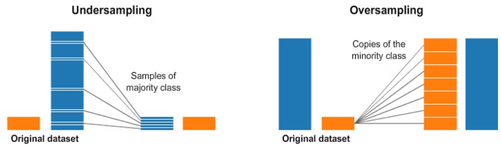
\includegraphics[width=0.8\linewidth]{16.png}
    %\fbox{\parbox[c][4cm][c]{0.8\linewidth}{\centering \textit{[Chèn ảnh: Minh họa Over-sampling (SMOTE / ADASYN) tại đây]}}}
    \caption{Các kỹ thuật cân bằng dữ liệu}
    \label{fig:balance_data}
\end{figure}

\begin{itemize}
    \item Mục đích: Làm cho dữ liệu đỡ bị mất cân bằng giữa các lớp.
    \item \textbf{Over-sampling:} Tăng mức độ tiếp xúc với phần dữ liệu thiểu số:
    \begin{itemize}
        \item \textbf{Nhân bản hóa (RandomOverSampler):} Nhân bản các thành phần thiểu số $\rightarrow$ số lượng tăng lên nhưng độ đa dạng không đổi.
        \item \textbf{Tổng hợp (SMOTE và ADASYN):}
        \begin{itemize}
            \item \textbf{SMOTE} (\textit{Synthetic Minority Oversampling Technique}): Hoạt động bằng cách chọn các điểm thuộc nhóm thiểu số gần điểm ban đầu, nội suy ra đường thẳng nối từ điểm $A$ đến điểm $B$ và chọn ngẫu nhiên một điểm nằm trên đường thẳng đó (trọng số của điểm mới dựa trên sự nội suy giữa $A$ và $B$).
            \item \textbf{ADASYN} (\textit{Adaptive Synthetic Sampling}): Hoạt động dựa trên việc sinh ra điểm nhân tạo từ các \textbf{điểm khó học} (điểm khó học là điểm bị bao quanh bởi nhiều điểm thuộc nhóm đa số $\rightarrow$ tính trọng số dựa trên các điểm đa số xung quanh, trọng số càng cao thì càng khó học; sau đó tiếp tục dùng kỹ thuật tương tự SMOTE để sinh ra điểm thiểu số nhân tạo).
        \end{itemize}
    \end{itemize}
    \item \textbf{Under-sampling:} Làm giảm phần dữ liệu đa số.
    \item $\rightarrow$ \textbf{Kết luận:} Chuộng \textbf{Over-sampling} hơn thay vì Under-sampling vì dữ liệu luôn cần được bảo toàn thay vì làm mất đi như Under-sampling.
\end{itemize}

% ==========================================
% SECTION 5: TRỰC QUAN HÓA DỮ LIỆU TRONG PYTHON
% ==========================================
\section{Data Visualization trong Python}

\begin{figure}[H]
    \centering
    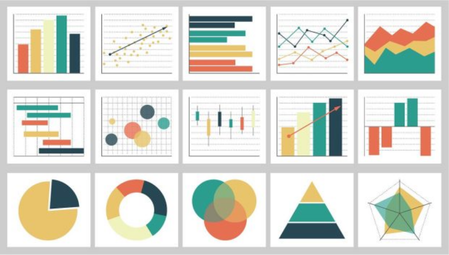
\includegraphics[width=0.8\linewidth]{17.png}
    %\fbox{\parbox[c][4cm][c]{0.8\linewidth}{\centering \textit{[Chèn ảnh: Các loại biểu đồ trực quan hóa dữ liệu tại đây]}}}
    \caption{Phân loại các biểu đồ trực quan hóa dữ liệu}
    \label{fig:data_vis}
\end{figure}

\begin{itemize}
    \item \textbf{Các thư viện phổ biến:} \texttt{numpy}, \texttt{matplotlib}, \texttt{pandas}, \texttt{seaborn}.
    \item \textbf{Các loại biểu đồ thường dùng:}
    \begin{itemize}
        \item Histogram
        \item Density plot (biểu diễn phân phối liên tục)
        \item Box plot
        \item Correlation matrix plot
        \item Scatter matrix plot
    \end{itemize}
    \item \textbf{Một số thành phần trong Matplotlib:}
    \begin{itemize}
        \item \texttt{grid}: Dóng cột và hàng (lưới tọa độ).
        \item \texttt{legend}: Chú thích (hữu ích khi một đồ thị có nhiều đường).
    \end{itemize}
\end{itemize}